\documentclass[12pt, a4paper]{scrartcl}

% --packages--
\usepackage[utf8]{inputenc}
\usepackage[italian]{babel}
\usepackage{graphicx}
\usepackage{MnSymbol}
\setlength{\parindent}{0pt}

\title{\textbf{Smart House}}
\author{735722 - Mattia Curatitoli\\ 737838 - Danilo Deponti} \date{}

\begin{document}
\maketitle
 
\section*{Introduzione}
L'invecchiamento della popolazione ha un impatto sempre più significativo sul sistema sanitario. Per questo si cercano vie più efficienti per portare assistenza in casa delle persone bisognose, in particolare gli anziani, il cui numero secondo le stime é in costante aumento grazie alle migliori condizioni di vita e di cure.

Monitorare le attività umane (\texttt{ADL}) è diventato un aspetto fondamentale per costruire un ambiente intelligente atto a garantire il benessere in grado di aumentare sia la sicurezza, sia l'autonomia dei soggetti.

Uno degli approcci più promettenti ed economici è il monitoraggio delle attività tramite una rete wireless di sensori (\texttt{WSN}) disposti nell'ambiente abitativo, in quanto molto flessibile e di facile sviluppo.
Sono stati sviluppati parecchi modelli che utilizzano sensori per monitorare le attività \texttt{ADL}, come ad esempio \emph{Reti Bayesiane} o \emph{Conditional Random Fields}. In particolare, si è notato che \emph{\textbf{Hidden Markov Model (HMM)}} è un modello performante in questo dominio applicativo; alcuni articoli approfondiscono il modello proponendo soluzioni di HMM ibridi, noi invece abbiamo implementato una versione classica.

\section*{I sensori}
Per costruire e testare il modello, sono stati utilizzati dataset presi da due appartamenti. Ogni appartamento fornisce due dataset: il primo con le rilevazioni generate dai sensori, il secondo con le attività rilevate dai sensori.
I sensori utilizzati sono stati di vario tipo (magnetici, a pressione, elettrici etc), disposti in più zone della casa in maniera il meno invasiva possibile e hanno registrato e salvato i dati per diversi intervalli di tempo (due settimane circa).

Il dataset delle rilevazioni sensoristiche (figura \ref{fig:dataset-sensori}) è una lista di righe corrispondenti all'intervallo di tempo nei quali i sensori sono stati attivi. Ogni riga é composta da: 
\begin{center}\begin{addmargin}[2em]{2em}
\texttt{Start time - End time - Location - Type - Place}
\end{addmargin}\end{center}
dove la tripla \texttt{Location-Type-Place} indica il sensore che ha effettuato la rilevazione.
\begin{figure}[!ht]
	\centering
	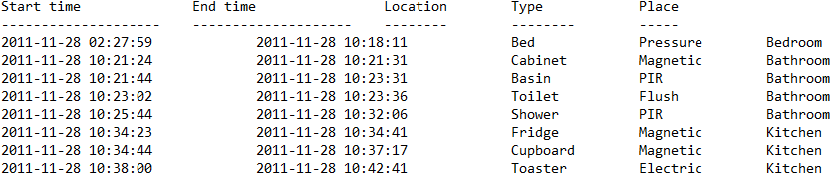
\includegraphics[scale=0.55]{Sensor.png} 
	\caption{Dataset dei sensori}
	\label{fig:dataset-sensori}
\end{figure}

Nel dataset delle attività ogni riga contiene l'intervallo di tempo e il nome dell'attività rilevata. 
Ogni attività è strettamente legata alla rilevazione effettuata dai sensori, ed é rappresentata (figura \ref{fig:dataser-activity}) su una riga come:
\begin{center}\begin{addmargin}[2em]{2em}
\texttt{Start time - End time - Activity}
\end{addmargin}\end{center}
\begin{figure}[!ht]
	\centering
	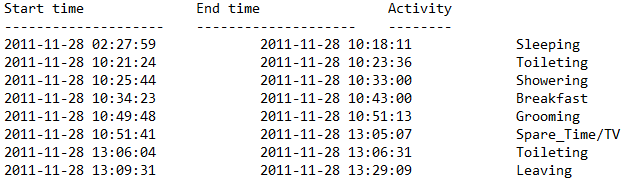
\includegraphics[scale=0.55]{Activity.png} 
	\caption{Dataset delle attività}
	\label{fig:dataser-activity}
\end{figure}

\section*{HMM}
Un \emph{HMM (Hidden Markov Model)} è un modello probabilistico definito da variabili osservabili $x_t$ e variabili nascoste $y_t$, dove $t$ indica il tempo. In questo caso le variabili osservabili sono i sensori, mentre le variabili nascoste sono le attività e dipendono come in figura \ref{fig:dependece-hmm}. 

In un \texttt{HMM} standard le variabili nascoste $y_t$ ($y$ al tempo $t$) dipendono solo dallo stato delle variabili $y_{t-1}$ ($y$ al tempo $t-1$), mentre le variabili osservabili $x_t$ ($x$ al tempo $t$) dipendono solo dallo stato delle variabili $y_t$ ($y$ allo stesso istante $t$).
\begin{figure}[!ht]
	\centering
	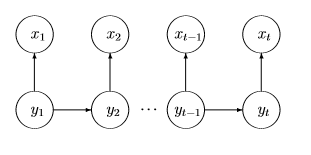
\includegraphics[scale=1]{HMM.png} 
	\caption{Dipendenze in un Hidden Markov Model}
	\label{fig:dependece-hmm}
\end{figure}

Necessari in un \texttt{HMM} sono: 
\begin{itemize}
\item i dati relativi a $p(y)$, ovvero la probabilità a priori delle variabili $y$; 
\item $p(y_t|y{_t-1})$ le probabilità di transizione da uno stato $y$ al successivo; 
\item $p(x_t|y_t)$ le probabilità di una variabile $x_t$ data $y_t$.
\end{itemize}

\section*{Il Software}
Il software è stato sviluppato in \texttt{Python}, e permette di creare un \texttt{HMM} partendo da una sequenza di rilevazioni prese dal dataset di un appartamento. 

Si è deciso di trasformare le rilevazioni dal formato testuale fornito \texttt{.txt} in un formato più compatto ed ordinato, il \texttt{csv}. Come verrà spiegato dettagliatamente nei successivi paragrafi, il software analizza i sorgenti del dataset e calcola le probabilità iniziali, di transizione degli stati e di emissione degli eventi in base alle occorrenze all'interno del file. Successivamente, il software si avvale di 2 librerie gratutite di nome \texttt{GHMM} e \texttt{Pomegranate}, in grado di creare modelli \texttt{HMM} e molte altre funzionalità, tra cui l'utilizzo dell'algoritmo di Viterbi.

Con \texttt{GHMM} é stato possibile solo costrutire il modello HMM, mentre con \texttt{Pomegranate} si é utilizzato l'algoritmo di Viterbi ed é stato possibile fare considerazioni sul modello creato.
Entrambi i modelli vengono però salvati in appositi file di testo generati a runtime.

\section*{Le librerie}
\subsection*{GHMM}
\texttt{GHMM} (General Hidden Markov Model) é una libreria gratuita, disponibile sotto licenza LGPL (GNU Lesser General Public License), scritta in C, ma disponibile in Python grazie a un wrapper che funge da interfaccia. Essa é in grado di costruire modelli base o estesi HMM con emissioni discrete o continue. 

É disponibile all'indirizzo \texttt{http://ghmm.org/} ed é sotto la supervisione del gruppo di ricerca di Alexander Schliep presso l'Università di Rutgers. Ha inoltre a disposizione una sezione all'indirizzo \texttt{http://sourceforge.net/projects/ghmm/} dove é possibile scrivere su un forum per eventuali richieste.

Presenta però due svantaggi:
\begin{itemize}
\item Non é frequentemente aggiornata e supportata (ultimo update 09/2015)
\item É facilmente installabile sono in ambiente Unix, in particolare sulla distibuzione Ubuntu; in ambiente OSX é molto complesso installarla a causa di diversi errori in fase di compilazione del sorgente in C; in ambiente Windows non é per niente supportata, ma solo disponibile attraverso l'utilizzo di Cygwin.
\end{itemize}

Per generare un HMM
\begin{center}\begin{addmargin}[2em]{2em}
\texttt{model = HMMFromMatrices(sigma, DiscreteDistribution(sigma), t\_adls, o\_sens\_adls, p\_adls)}
\end{addmargin}\end{center}

con il dizionario delle emissioni \texttt{sigma}
\begin{center}\begin{addmargin}[2em]{2em}
\texttt{sigma = IntegerRange(0, len(list\_sens))}
\end{addmargin}\end{center} 

e con \texttt{t\_adls} matrice delle transizioni, \texttt{o\_sens\_adls} matrice delle osservazioni e \texttt{p\_adls} lista delle probabilità a priori delle variabili nascoste.

\subsection*{Pomegranate}
\texttt{Pomegranate} é una libreria per Python, implementata in Cython (un compilatore C per Python), nata dal pre-esistente, e non piú supportato, progetto \texttt{YAHMM}, che permette la gestione di reti Bayesiane, Catene di Markov, HMM, Macchine a stati finiti e altro ancora. 

É disponibile la documentazione ben aggiornata all'indirizzo \\ \texttt{http://pomegranate.readthedocs.io/en/latest/} ed é facilemnte installabile tramite il pacchetto \texttt{pip} eseguendo da terminale 
\begin{center}\begin{addmargin}[2em]{2em}
\texttt{pip install pomegranate}
\end{addmargin}\end{center}

Per generare un HMM
\begin{center}\begin{addmargin}[2em]{2em}
\texttt{model = HiddenMarkovModel( name="Model-name" )}
\end{addmargin}\end{center}

Il package caratterizza ogni stato nascosto e le sue emissioni con la seguente sintassi:
\begin{center}\begin{addmargin}[2em]{2em}
\texttt{ADL1 = State( DiscreteDistribution({ 'sens1': 0.1, 'sens2': 0.4, 'sens3': 0.5 }), name='ADL1' )}
\end{addmargin}\end{center}

Dopodichè, è necessario definire le probabilità iniziali come segue:
\begin{center}\begin{addmargin}[2em]{2em}
\texttt{model.add\_transition( model.start, ADL1, 0.6 )}
\end{addmargin}\end{center}

e le probabilità di transizione tra gli stati nel seguente modo:
\begin{center}\begin{addmargin}[2em]{2em}
\texttt{model.add\_transition( ADL1, ADL2, 0.65 )}
\end{addmargin}\end{center}

Successivamente, dopo la chiamata \texttt{model.bake()} che permette l'effettiva elaborazione dei dati forniti per la creazione del \texttt{HMM}, è possibile fare diversi tipi di inferenze sul modello. Come \texttt{forward},\texttt{backward}, \texttt{forward-backward} e \texttt{Viterbi}.

\section*{Le funzioni}
Di seguito sono descritte le funzioni principali del software, in modo da illustrare dettagliatamente il metodo usato per creare le probabilità utilizzate per la creazione del modello.

\subsection*{check\_and\_generate\_csv}
Prende in input il path di un file testuale \texttt{.txt} ed esamina riga per riga (evitando le prime due che nel dataset fornito sono di intesazione) e per ognuna verifica che lo \texttt{Start time} sia antecedente al \texttt{End time}; sono stati anche implementati, ma non funzionanti, i controlli tra gli \texttt{Start time} e \texttt{End time} tra righe consecutive. Se non sono presenti errori genera un file \texttt{.csv} con i dati controllati, altrimenti lancia un messaggio di errore che indica in quale righe sono state rilevate incorrettezze.

Questo controllo ci ha permesso di scoprire un errore nel file originale rispetto alcuni \texttt{Start} e \texttt{End time}
\begin{figure}[!ht]
	\centering
	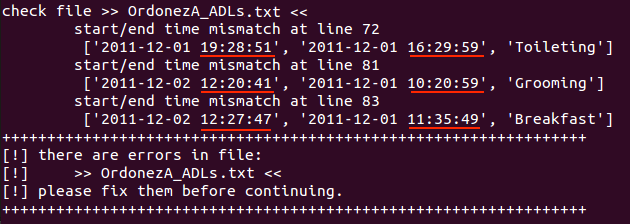
\includegraphics[scale=0.6]{error.png} 
	\label{fig:error}
\end{figure}

\subsection*{normalize\_list e normalize\_matrix}
Queste funzioni prendono in input rispettivamente liste e matrici e normalizzano i dati contenuti, utilizzando la divisione fornita della libreria \texttt{numpy}. In questo modo ogni lista e ogni riga della matrice ha come somma $1.0$.

\subsection*{csv\_list e csv\_matrix}
Come facilmente intuibile, generano file in formato \texttt{.csv} a partire dai dati in input: lista dei nomi delle variabili (su righe e colonne per la matrice) e lista (o matrice) dei valori da inserire.

\subsection*{obtain\_p\_adls}
Permette di ricavare la lista delle attività rilevate, le probabilità iniziali di ogni singola attività e la sequenza di attività presente nel dataset. Questa funzione prende in input il percorso del file csv contenente le attività da analizzare e semplicemente conta le occorrenze di ciascuna stessa attività all'interno del file incrementando un contatore ad ogni rilevazione, dopodichè normalizza i dati.

\subsection*{obtain\_t\_adls}
Permette di ricavare la matrice delle transizioni per le \texttt{ADLs}. Conta, ogni volta che un attività accade al tempo $t$, quante volte ogni singola attività compare al tempo $t-1$, in modo da generare una matrice $n\times n$ con la somma, per ogni attività, delle volte che le altre attività sono accadute successivamente. Infine normalizza i dati.

\subsection*{obtain\_list\_sens}
A partire dal file in input ricava la lista dei sensori attivati durante le rilevazioni (composti dalla tripla univoca \texttt{Location-Type-Place}) e la sequenza con cui sono stati attivati.

\subsection*{obtain\_o\_sens\_adls}
La funzione permette di ricavare le probabilità di emissione dalle \texttt{ADLs} ai sensori. Viene tenuto conto di tutte le volte che l'intervallo di tempo di una rilevazione del sensore cade all'interno della rilevazione di un'attività. La matrice ottenuta é poi normalizzata.

\section*{Esecuzione e stime}
Da ogni dataset vengono calcolate le matrici di transizione degli stati nascosti, di osservazione e le probabilità a priori e dati in pasto alla libreria pomegrante, la quale genera il modello come descritto in precedenza.

Una volta generato il nostro modello, utilizzeremo \emph{l'algoritmo di Viterbi} con il comando 
\begin{center}\begin{addmargin}[2em]{2em}
\texttt{model.viterbi(sequence)}
\end{addmargin}\end{center}

dove \texttt{sequence} é la sequenza di sensori fornita dal dataset. 

Esso genera la sequenza di attività ottima generata in base alla \texttt{sequence} inserita; in questo modo possiamo verificare se la sequenza di \texttt{ADLs} risultante è coerente con quella della fornita dal dataset originale.

\subsection*{Parametri di affidabilità}
Per ricavare informazioni dal confronto tra la sequenza di attività orginale (che chiamiamo per semplicità \texttt{seq1}) e quella generata a partire dal modello HMM (che chiamiamo \texttt{seq2}) abbiamo implementato tre differenti metodi.

\subsubsection*{diff\_base}
Calcola un rate in base alla differenza punto-a-punto tra le due sequenze inserite; il punteggio ideale é prossimo allo zero, poiché:
\begin{itemize}
\item inizializzo un contatore di diff a zero
\item ogni volta che le \texttt{ADLs} tra le due sequenze alla stessa posizione non sono uguali incremento di \texttt{1} un contatore 
\item calcolo il rapporto tra il numero di diff e la lunghezza della sequenza di riferimento \texttt{seq1}
\end{itemize}
quindi più il rapporto é vicino allo zero, meno sono le differenze punto-a-punto tra le due sequenze.

\subsubsection*{diff\_A} 
Assegna un rate in base all'uguaglianza o meno tra un'attività al passo $x$ di \texttt{seq1} e l'intervallo attorno al passo $x$ di \texttt{seq2}.
\begin{itemize}
\item inizializzo un contatore di diff a zero
\item ogni volta confronto la \texttt{ADL} in posizione $x$ di \texttt{seq1} con le \texttt{ADL} nell'intervallo attorno a $x$ in \texttt{seq2}
\item assegno un punteggio alla distanza dal centro dell'intervallo (\texttt{0} se il match é in posizione $x$, 1 se il match é in $x+1$ o $x-1$ e così via 
\item calcolo il rapporto tra il rate ottenuto e la lunghezza della sequenza di riferimento \texttt{seq1}
\end{itemize}
Più il rapporto é prossimo allo zero, migliore é la somiglianza tra le due sequenze.

\subsubsection*{diff\_B}
Assegna un rate in base allo scostamento dei match tra le due sequenze;
\begin{itemize}
\item ad ogni passo confronto la \texttt{ADL} in $x$ della \texttt{seq1} e scorro la \texttt{seq2} fino a quando non trovo un match in $y$
\item il passo successivo cerca il match tra $x+1$ della \texttt{seq1} a partire da $y+1$ della \texttt{seq2}
\item calcolo il rapporto tra la lunghezza della sequenza di riferimento \texttt{seq1} con il punto di arrivo in \texttt{seq2}
\end{itemize}
Più il rapporto é vicino ad \texttt{1} e più le due sequenze sono simili e intervallate da poche differenze.

\subsection*{Conclusioni e sviluppi futuri}
Le analisi sono fatte su ogni singolo dataset (ovvero appartamento) fornito e dai risultati ottenuti si può dire che:
\begin{itemize}
\item a partire dal modello costruito su \emph{OrdonezA}, si ottiene una sequenza di attività abbastanza diversa putno-a-punto da quella originale, ma con poche differenze se si considerano gli \emph{intorni} e la sequenza complessiva scartando eventuali \emph{dati sporchi} (figura \ref{fig:ordonezA})
\item a partire dal modello costruito su \emph{OrdonezB}, si ottiene una sequenza di attività ancora più differente putno-a-punto da quella originale, ma con poche differenze se si considerano gli \emph{intorni} e ancora meno se si considera la sequenza complessiva scartando i \emph{dati sporchi} (figura \ref{fig:ordonezB})
\end{itemize}

\begin{figure}[!ht]
	\centering
	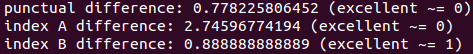
\includegraphics[scale=0.6]{ordonezA.png} 
	\caption{output OrdonezA}
	\label{fig:ordonezA}
\end{figure}
\begin{figure}[!ht]
	\centering
	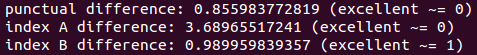
\includegraphics[scale=0.6]{ordonezB.png} 
	\caption{output OrdonezB}
	\label{fig:ordonezB}
\end{figure}

Per migliorare i risultati potrebbe essere interessante approfondire l'associazione tra rilevazioni sensoristiche ravvicinate e simili, che sono identificate da un'unica attività. Si nota infatti che la nostra sequenza di \texttt{ADLs} generata con l'algoritmo di Viterbi, nonostante venga \emph{ripulita} da ripetizioni di attività non significative, si presenta comunque più lunga rispetto alla sequenza originale, proprio perchè va a generare un attività a partire da ogni rilevazione da sensore, a differenza dell'output fornito dal dataset.

Sarebbe anche interessate integrare con tool grafici disponibili con la libreria \texttt{Pomegranate} per poter indagare anche ad occhio nudo i procedimenti dell'algoritmo.

Un altra possibilità, avendo a disposizione un dataset di maggiori dimensioni, potrebbe essere di indagare l'attendibilità di previzione di \texttt{ADLs} non solo per ogni appartamento singolo, ma per un insieme di appartamenti, e magari inferire eventuali differenze.

\end{document}
